\documentclass[dvipsnames,
%xcolor={svgnames},
hyperref={
	citecolor=blue,
	colorlinks=true,
	urlcolor=blue,
	linkcolor=,
}
]{beamer}
\beamertemplatenavigationsymbolsempty
\usetheme{Boadilla}
\usefonttheme[onlymath]{serif}

\usepackage{cleveref}

\usepackage{amsmath}
\usepackage{bm}
\usepackage{bbm}
\usepackage{mathrsfs}
\usepackage{mathtools}
\usepackage[cal=boondoxo]{mathalpha}

% Change horizontal spacing
\setlength{\tabcolsep}{3pt}

\usepackage[none]{hyphenat} % no hyphenation

\usepackage{array}

\usepackage{cancel}

\usepackage[style=authoryear,maxcitenames=2,backend=biber,citetracker=true]{biblatex}
\addbibresource{references.bib}

\usepackage{verbatim}

\usepackage{bigints}

\usepackage{makecell}

\usepackage{subcaption}

\DeclareCiteCommand{\citeauthor}
{\boolfalse{citetracker}%
	\boolfalse{pagetracker}%
	\usebibmacro{prenote}}
{\ifciteindex
	{\indexnames{labelname}}
	{}%
	\printtext[bibhyperref]{\printnames{labelname}}}
{\multicitedelim}
{\usebibmacro{postnote}}

\DeclareCiteCommand{\citeyear}
{\usebibmacro{prenote}}
{\bibhyperref{\printfield{year}}\bibhyperref{\printfield{extrayear}}}
{\multicitedelim}
{\usebibmacro{postnote}}

\newcommand{\credit}[2]{{\par\hfill \tiny #1 credit:~\itshape{\color{blue} \citeauthor{#2} (\citeyear{#2})}}}
\newcommand{\crediturl}[2]{{\par\hfill \tiny #1 credit:~\itshape{\color{blue} \url{#2}}}}
\let\oldcite\cite
\renewcommand{\cite}[1]{{\color{blue} \oldcite{#1}}}
\newcommand{\citefoot}[1]{{\color{blue} \citeauthor{#1} (\citeyear{#1})}}
\newcommand{\matr}[1]{#1}

\newcommand{\red}[1]{{\color{red} #1}}

\title[Deep Imbalanced Regression]
{\href{https://doi.org/10.48550/arXiv.2102.09554}{Deep Imbalanced Regression}}
%\subtitle{}
\author[Yang Y. et al.]{Yang Y, Zha K, Chen Y, Wang H, Katabi D}
%\institute{Aalto University}
\date{}%3 July 2024}

\addtobeamertemplate{title page}{}{
\begin{center}
\vspace{-5em}
ICML 2021
\\\vspace{4em}Presenter: Gianmarco Midena
\\\vspace{1em}26 November 2024
\end{center}}

\begin{document}
	
\begin{frame}[noframenumbering,plain]
\titlepage
\end{frame}

\begin{frame}{Overview}
	\begin{figure}[h]
		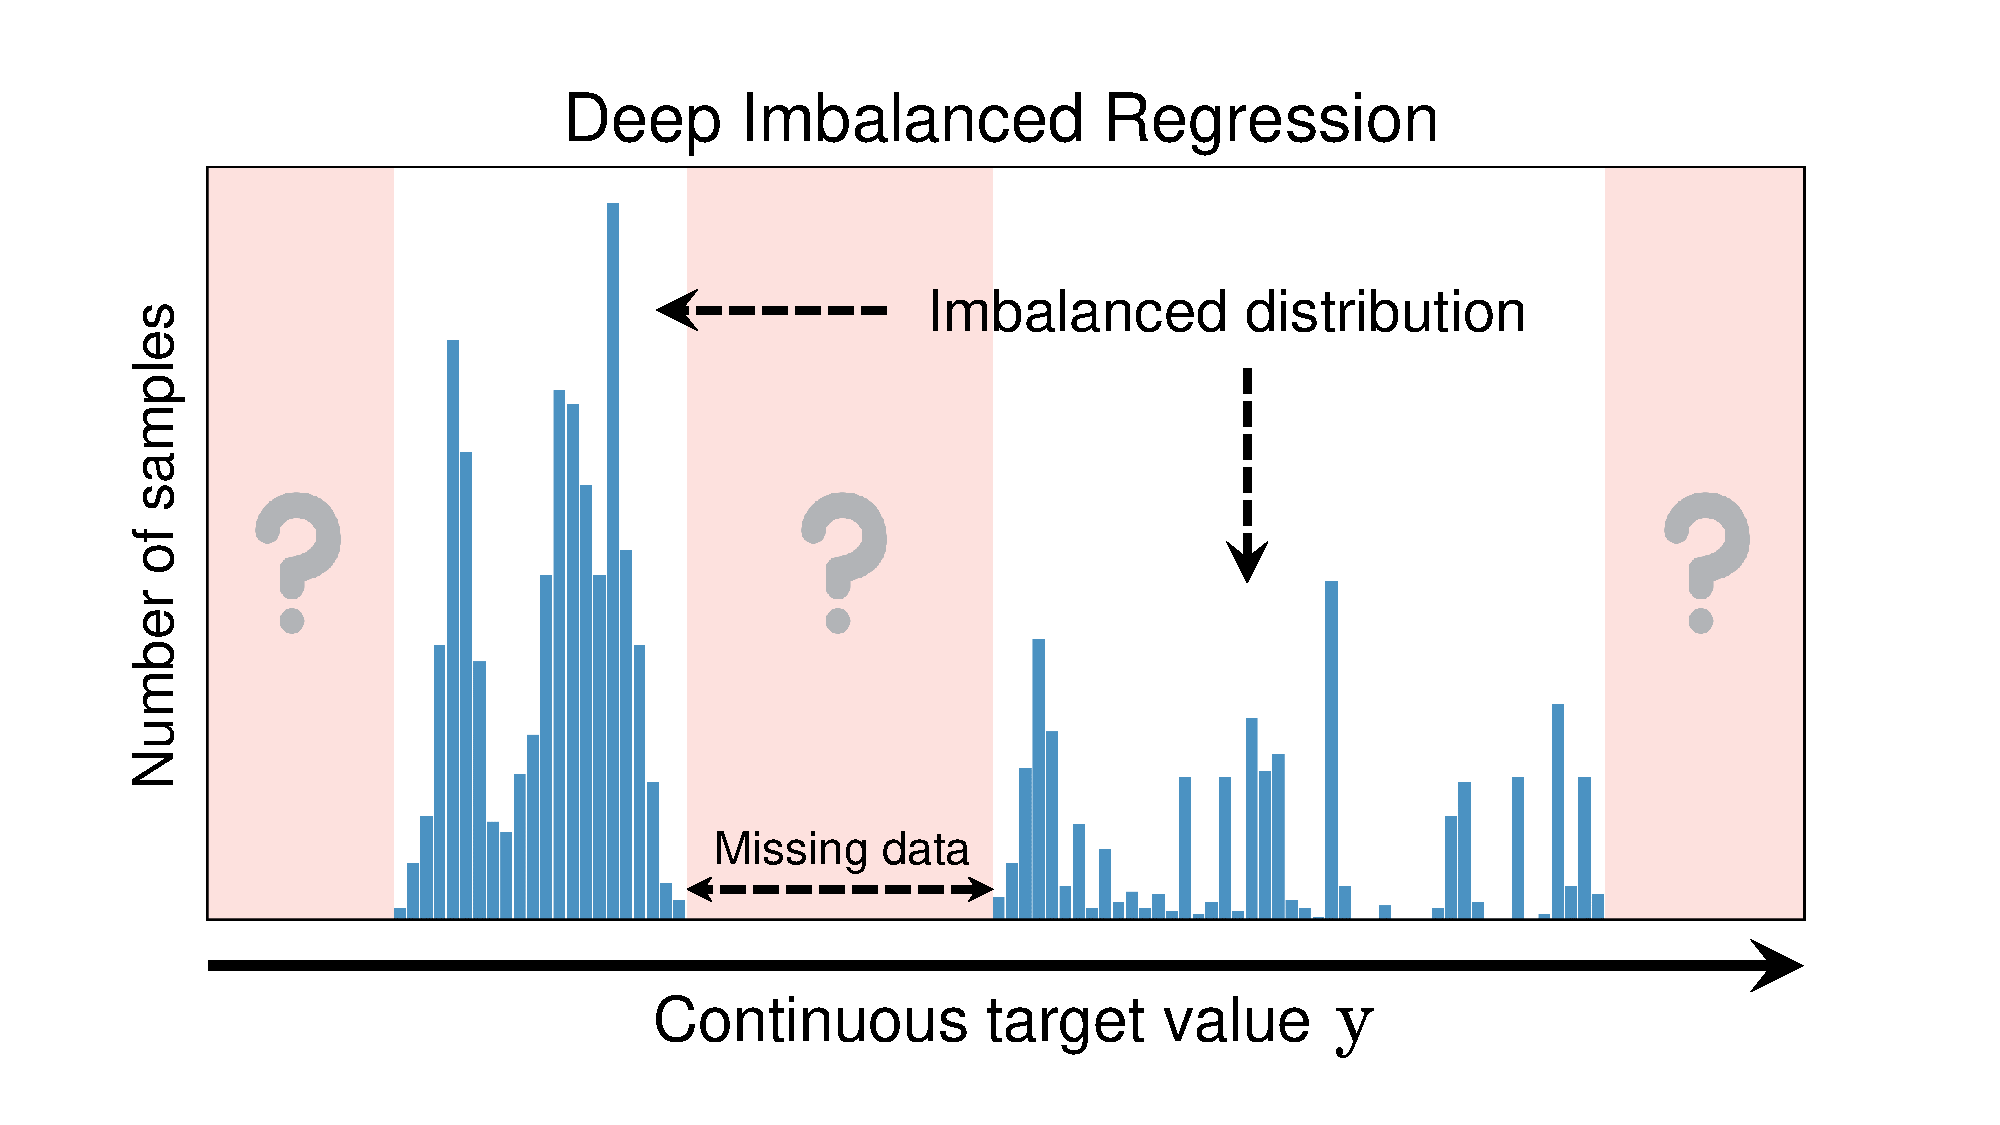
\includegraphics[width=\linewidth]{images/teaser.pdf}
		%\caption{}
	\end{figure}
	\credit{Image}{yang2021delving}
\end{frame}

\begin{frame}{Test Error on Categorical vs. Continuous Label Space}
	\begin{figure}[h]
	\begin{subfigure}{0.48\textwidth}
		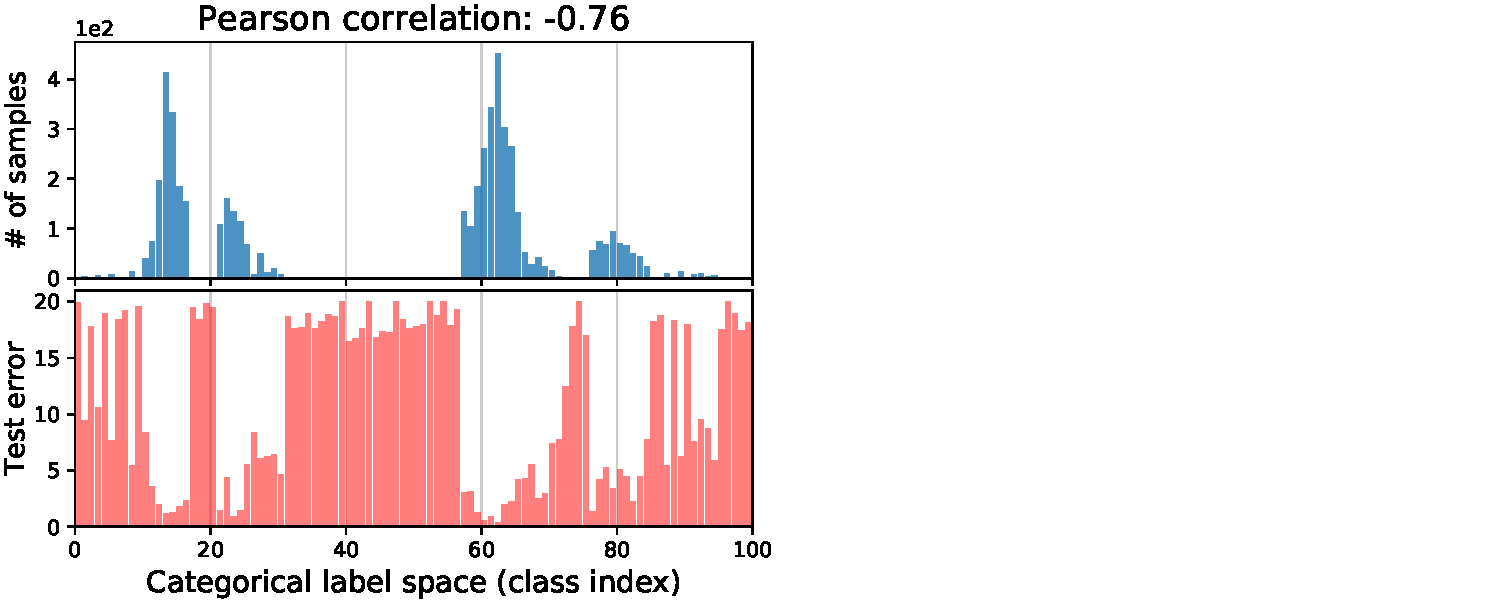
\includegraphics[width=\linewidth]{images/err_motivate_1_left.pdf}
		\caption{CIFAR-100 (subsampled)}
	\end{subfigure}\hspace{1em}%
	\begin{subfigure}{0.48\textwidth}
		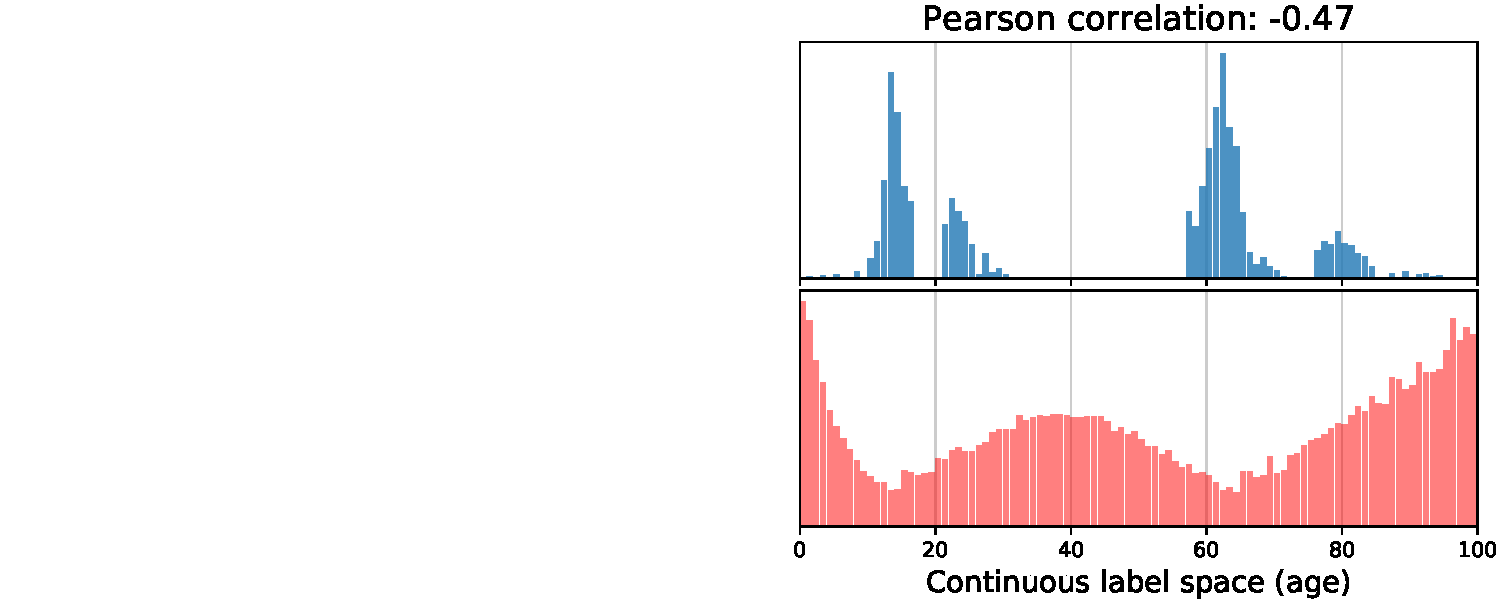
\includegraphics[width=\linewidth]{images/err_motivate_1_right.pdf}
		\caption{IMDB-WIKI (subsampled)}
	\end{subfigure}
	%\caption{}
	\end{figure}
	\credit{Image}{yang2021delving}
\end{frame}

\begin{frame}{Problem Settings}
	\begin{itemize}
		\item $\{(\mathbf{x}_i, y_i)\}_{i=1}^N$: training set
		\item $\mathbf{x}_i\in\mathbb{R}^{d}$: input
		\item $y_i\in\mathcal{Y}$: continuous label or target
		\item $b_i\in\mathcal{B}$: discrete label or target
		\item $\mathcal{Y}\subset\mathbb{R}$: continuous label space
		\item $\mathcal{B} = \{1,\dots,M\}\subset\mathbb{Z}^+$: index space
		\begin{itemize}
			\item divides $\mathcal{Y}$ into $M$ groups (bins) with equal intervals $[t_j, t_{j+1})$
			\item $\{[t_0, t_1), \dots, [t_{M-1}, t_M)\}$: discrete label space
			\item $t_k\in\mathcal{Y}$
			\item minimum resolution
			\begin{itemize}
				\item e.g., $\delta y \triangleq t_{j+1} - t_j = 1$ in age estimation
			\end{itemize}	
		\end{itemize}
		\item $\hat{y}_i = g(\mathbf{z}_i) \in \mathbb{R}$: predicted continuous label
		\item $\mathbf{z}_i = f(\mathbf{x}_i; \theta) \in \mathbb{R}^{d'}$: learned representation
		\item $\theta$: trainable model parameters
	\end{itemize}
\end{frame}

\begin{frame}{Label Distribution Smoothing}
	\begin{figure}[h]
		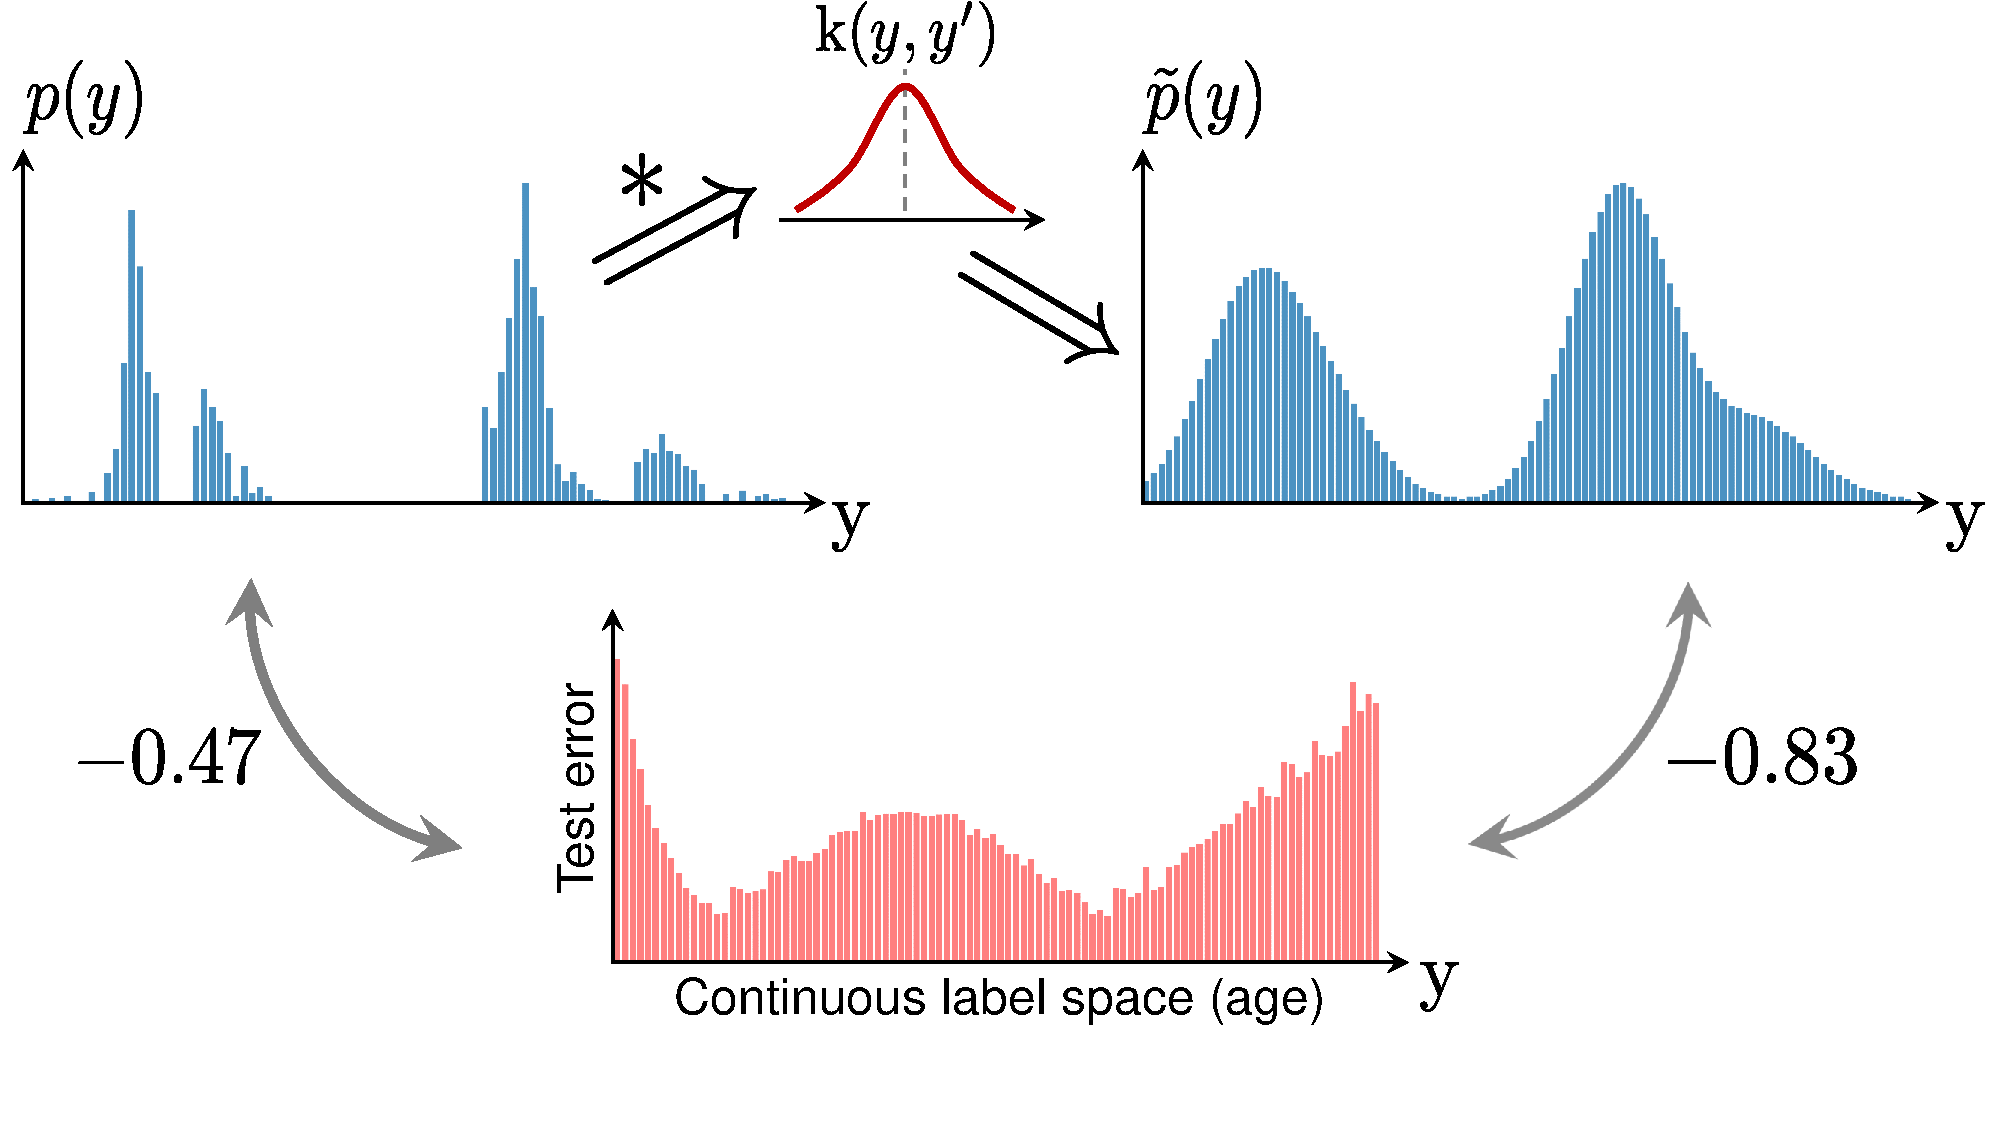
\includegraphics[width=\linewidth]{images/err_motivate_sep.pdf}
		%\caption{}
	\end{figure}
	\credit{Image}{yang2021delving}
\end{frame}

\begin{frame}{Feature Distribution Smoothing}
	\begin{figure}[h]
		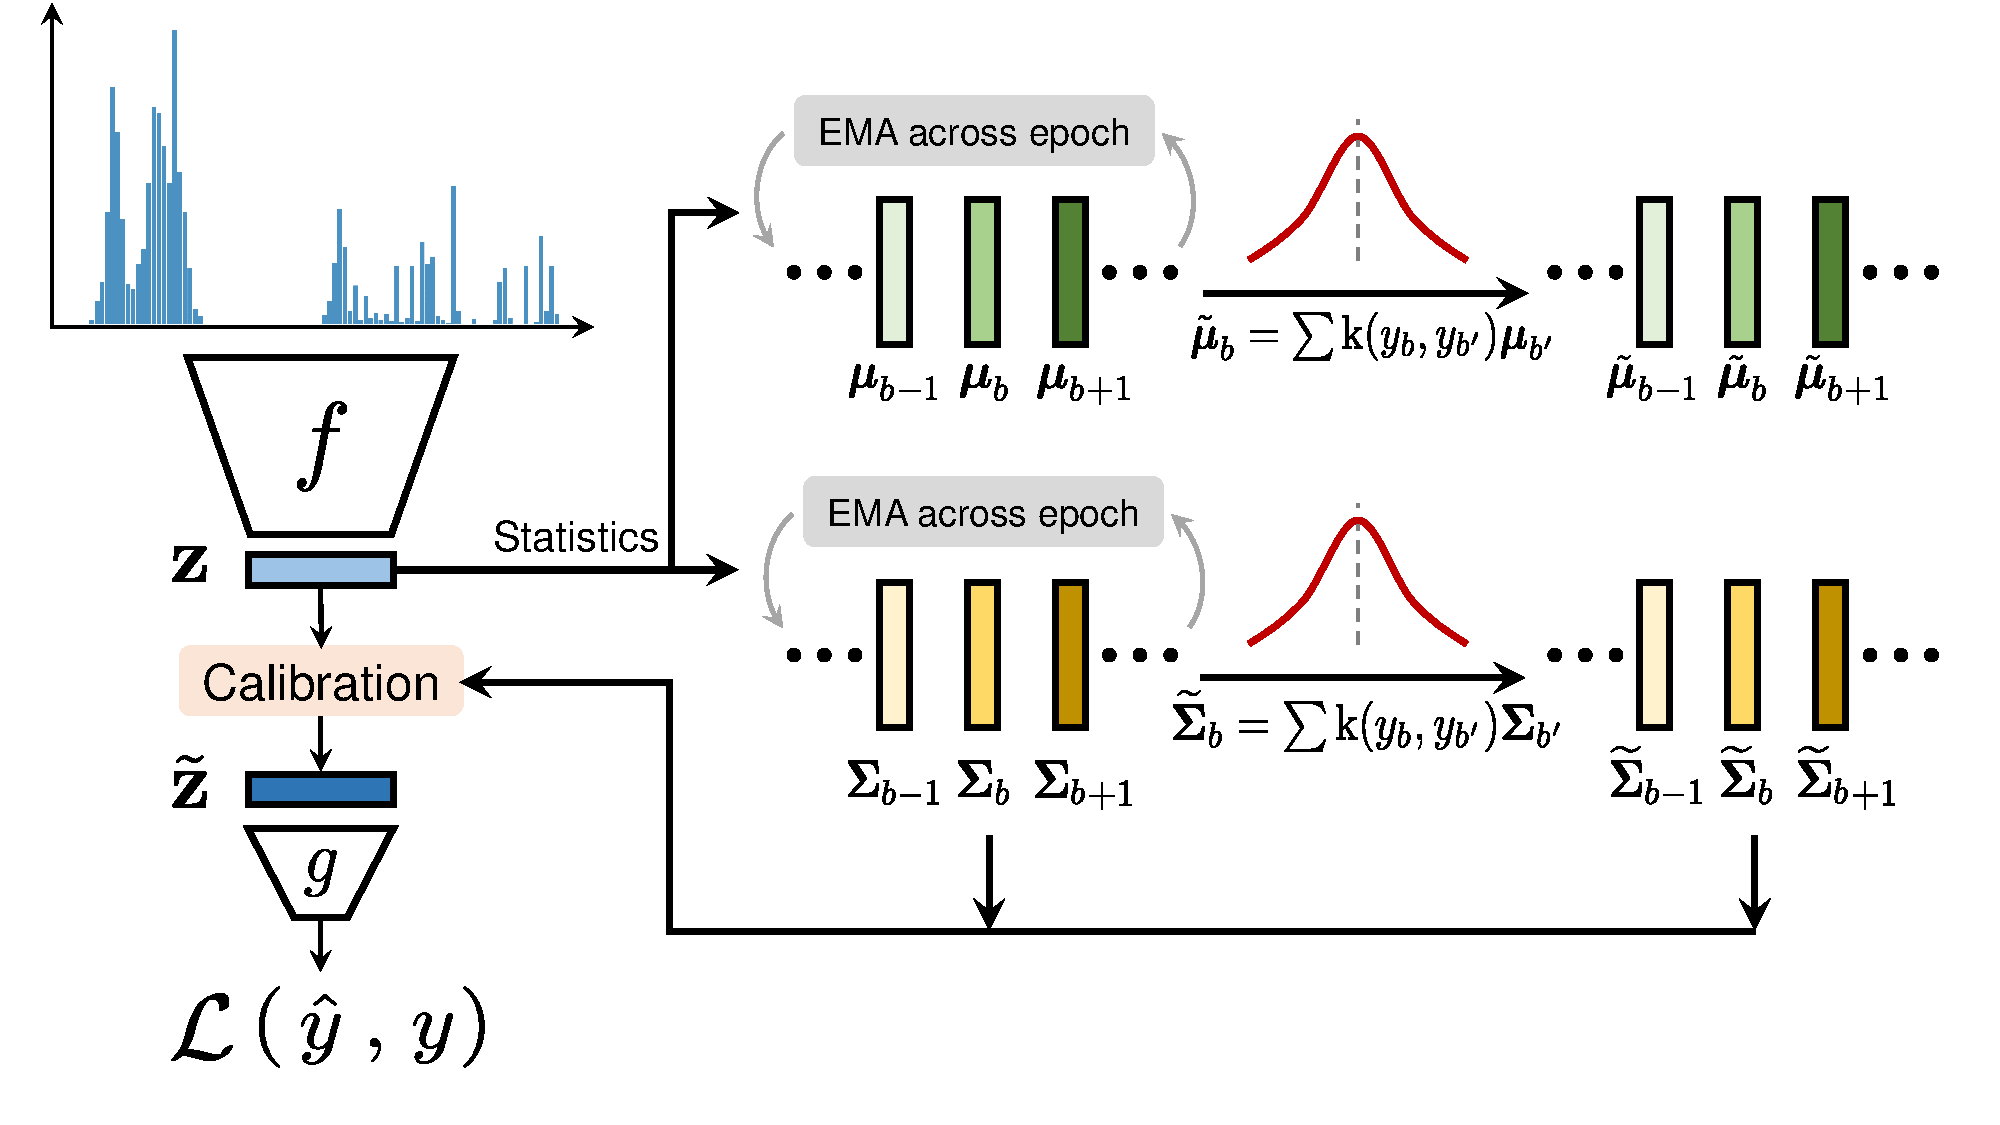
\includegraphics[width=\linewidth]{images/teaser_fds.pdf}
		%\caption{}
	\end{figure}
	\credit{Image}{yang2021delving}
\end{frame}

\begin{frame}{Baselines (1/2)}
	\begin{enumerate}\setlength\itemsep{1.5em}
		\item<1-> Vanilla: neglects data imbalance
		\item<2-> Synthetic samples
		\begin{itemize}
			\item SMOTER (\cite{torgo2013smote})
			\begin{enumerate}
				\item Defines frequent and rare regions using label density.
				\item Creates synthetic samples for pre-defined rare regions by linearly interpolating both inputs and labels.
			\end{enumerate}
			\item SMOGN (\cite{branco2017smogn}): augments SMOTER with Gaussian noise
		\end{itemize}
		\item<3-> Focal-R
		\begin{equation*}
			\frac{1}{n} \sum_{i=1}^n \sigma(|\beta e_i|)^\gamma e_i
		\end{equation*}
		\begin{itemize}
			\item Error-aware loss
			\item Maps absolute error into $[0, 1]$.
			\item $e_i$: $L_1$ error for $i$-th sample
			\item $\beta$, $\gamma$: hyper-parameters
			\item Inspired by Focal Loss (\cite{lin2017focal}) for classification
		\end{itemize}
	\end{enumerate}
\end{frame}

\begin{frame}{Baselines (2/2)}
	\begin{enumerate}\setcounter{enumi}{3}\setlength\itemsep{1.5em}
		\item<1-> Regressor re-training (RRT)
		\begin{itemize}
			\item Two-stage training
			\begin{enumerate}
				\item Train encoder
				\item Re-train regressor with inverse re-weighting and frozen encoder.
			\end{enumerate}
			\item Inspired by \cite{kang2019decoupling}
		\end{itemize}
		\item<2-> Cost-sensitive re-weighting: re-weighting schemes based on label distribution
		\begin{itemize}
			\item Inverse-frequency weighting (INV)
			\item Square-root weighting variant (SQINV)
		\end{itemize}
	\end{enumerate}
\end{frame}

\section{References}
\begin{frame}[noframenumbering,plain]%[allowframebreaks]
\frametitle{References}
\printbibliography
\end{frame}

\end{document}